\section{User Study: Trust Evaluation}
In the previous section, we discussed three systems with different accuracy levels and three types of explanations. Similar to the experiment discussed in \cite{langer1978mindlessness}, we have built a system offering (1) no explanation for its decision, (2) a placebic explanation (non-informative) for its decision, and (3) an informative (i.e. truthful) information for its decision. In this section we present the user study in which we investigated the influence of model accuracy and explanation fidelity on user trust. We use two approaches to measure user trust: an explicit measure based on a questionnaire and a proxy that measures trust via the willingness to accept and adapt to the system's recommendations.


\subsection{Method}

\paragraph{Participants}
In total, 327 participants took part in the main user study with an average age of 29.4 years (SD = 8.8), a gender balance of 56\% (males) to 43\% (females) and two participants reporting the third gender. 87\% of the participants were recruited via the paid science crowdsourcing platform ``Prolific", while 36 participants enlisted on ``SurveyCircle", an unpaid participant recruitment platform based on mutuality.\newline
On both platforms, individuals younger than 18 years were excluded to participate for reasons of consent by a major. The use case scenario included reading and understanding real-life Tweets with slang words, grammatical and literal errors. The platforms therefore screened for people being fluent in English. 57\% self-assessed their level of English to be equivalent to a native speaker, 23\% as advanced (C1 on the Common European Framework of Reference for Language scale \cite{council2001common}), 14\% as upper-intermediate (B2), and 5\% as lower than that. All participants claimed to be ``fluent" in English. The study questionnaire included an attention check question, asking the participants to answer ``completely disagree" in between the trust questionnaire items assessed on a 5-point Likert scale. Data from participants who failed to answer the attention check correctly was excluded from the analysis. Furthermore, only complete responses were used in the analysis, i.e. data from participants who reached the last page of the survey. The exclusion criteria invalidated 41 data points, resulting in 286 valid cases.\newline
All participants recruited on the paid platform ``Prolific" received a compensation of 1.40 GBP (1.60 EUR) for an estimated completion time of 12 minutes. Participants from ``SurveyCircle" received a reward of 4.4 Study Points.

\paragraph{Apparatus}
The user study was set up as an online study, the study could therefore be taken at a self-chosen location on private devices. Participants were asked to completed the survey on a notebook, desktop computer or tablet. For consistency with the use case scenario, screenshots of a fictive social media management platform showed the input texts, decisions and explanations. The screenshots had a ratio of 900px (width) to 253px (height). To ensure that improper scaling of the screenshots did not influence the participants' perception, devices with small screens (e.g. smartphones and other mobile devices) were excluded. However, which device participants finally used could not be verified. No further requirements were made regarding the equipment of the participant's device.

\paragraph{Procedure}
On both platforms, the participants receive a link to the survey. As soon as the participant has opened the survey URL, the survey starts. The survey consists of the following content:
\begin{enumerate}
	\item Introduction \& consent form
	\item \textit{Scenario 1}: Social media administrator and manual offensive language detection
	\item \textit{Tweet block 1}: 15 Tweets for classification, on individual pages (no system)
	\item \textit{Scenario 2}: Introduction to automatic decision system supporting the task
	\item \textit{Tweet block 2}: Repetition of 15 Tweets for classification, on individual pages (with system)
	\item Perceived understanding \& trust questionnaire
	\item Demographics
	\item Outroduction \& crowdsourcing completion codes
\end{enumerate}
In general, the study contains three blocks plus an introduction and outroduction section. The first block treats a scenario in which the participant plays the role of a ``social media administrator" of a company with a young target group (15-20 years old). The task of the social media administrator is to identify content with offensive language in order to block such comments or Tweets. The next 15 pages of the survey contain one Tweet each, shown on a screenshot of a management tool, and ask the participant to classify the text as offensive or not offensive as shown in figure \ref{fig:survey_tools1}. The order in which the Tweets are shown is randomised for each participant. There are 10 different sets of Tweets available (without overlap), to avoid effects from the specific wording or topics in the small set of 15 Tweets. At the start of the survey, each participant is randomly assigned to one Tweet set by the system.\newline
\begin{figure} [H]
	\centering
	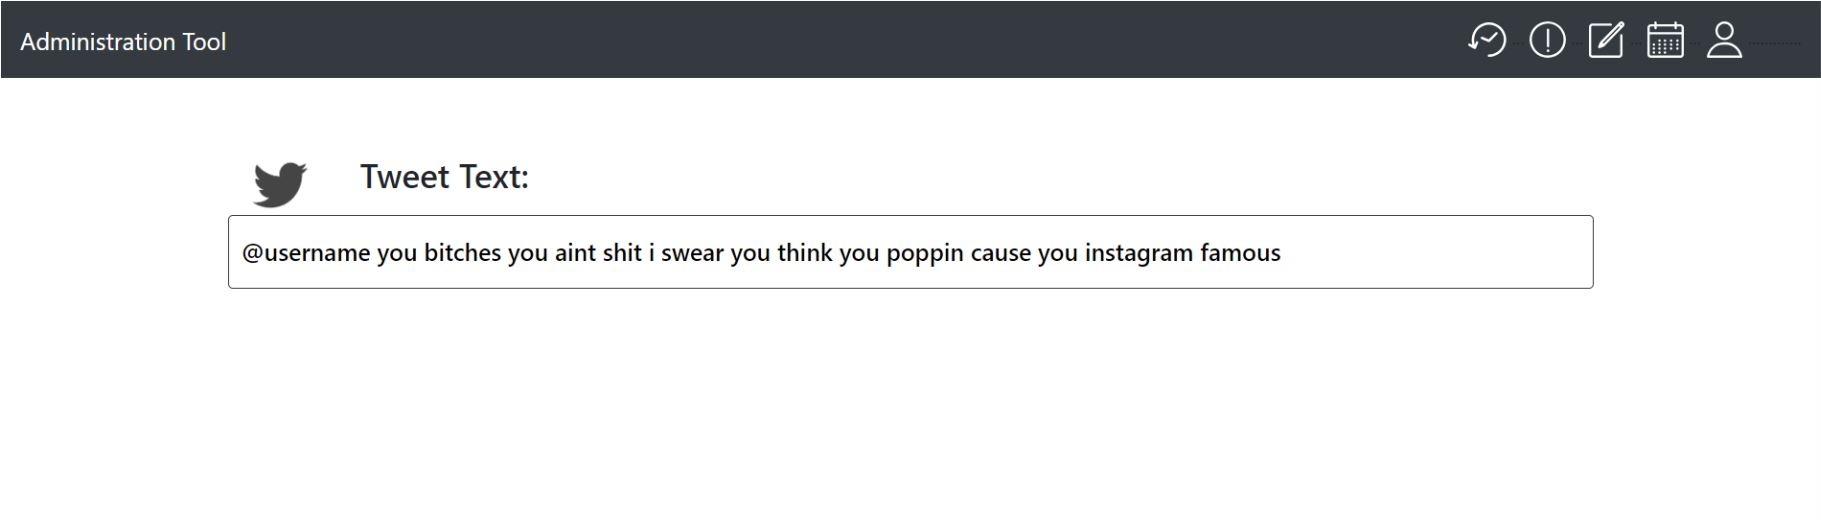
\includegraphics[width=0.8\textwidth]{img/neu_5_13.JPG}\\
	\caption{Screenshot of the fictive management tool without the automatic decision system}
	\label{fig:survey_tools1}
\end{figure}
The second block introduces the automatic decision system (see figure \ref{fig:survey_tools2}). The participant is again asked to classify 15 ``very similar" Tweets, which are, in fact, identical to the ones shown in the first block. This particular formulation aims to liberate the participants from the urge to classify each text with exactly the same label as in the first block. The ordering of the Tweets is random and hence very likely to be different from the ordering of the first block. In total, 9 conditions exist: three systems (classifier with 0.95, 0.75, and 0.05 accuracy) with three explanation types (informative, placebic, no explanation) each. Each participant has one condition assigned at the beginning of the survey, such that there is an equal distribution of conditions in finished questionnaires. \newline
\begin{figure} [H]
	\centering
	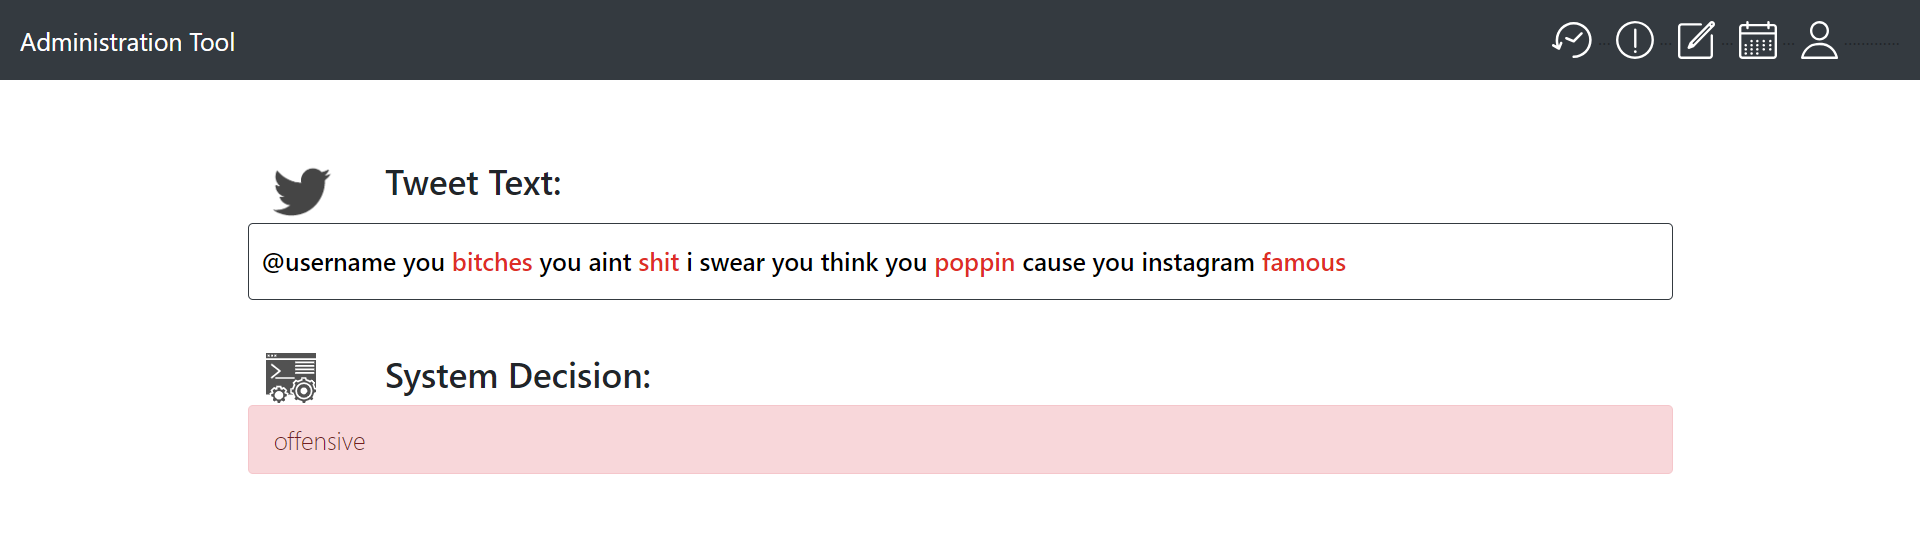
\includegraphics[width=0.8\textwidth]{img/pg_5_13.PNG}\\
	\caption{Screenshot of the fictive management tool with the automatic decision system}
	\label{fig:survey_tools2}
\end{figure}
Finally, the last block contains three questions regarding perceived understanding, 19 items measuring the user's trust including an attention check, and 5 demographic questions (gender, age, country, ethnicity, English language level).

\paragraph{Design \& Analysis}
The between-subject setup described in the previous paragraph was tested in a pilot study with 11 participants. The participants were recruited via ``Prolific" and received a compensation of 2.00 GBP (2.28 EUR). They completed the study in ``pretest" mode, which shows an additional comment box at the bottom of each survey page.\newline
The main study was set up as a quantitative study without open questions or free text input. Basic frequency analysis was used for the demographic items in order to understand the background of the participants. Three topics were investigated in a statistical manner: perceived understanding (3 items), self-reported trust (19 items), and observed trust via proxy. For the first two, a 5-point Likert scale was employed.\newline
A \textit{Perceived understanding} score was calculated for each participant by taking the mean of the ratings for all three items in the questionnaire. The trust questionnaire used to measure \textit{self-reported trust} contains 14 positive items and 5 inverse items. A single mean score was calculated by taking the average over the positive items and the maximum rating minus the mean of the inverse items. As a second trust measure, \textit{observed trust} was investigated via the proxy of willingness to follow a system's recommendation. The survey contained one block of manual classification without the system, and a second round with the information provided by the automated decision system. In each block, participants classified the same set of Tweets. We can therefore determine how often a participant switched his or her classification out of 15 possible cases and how often the change was made in agreement with the classifier's prediction but against the truth. Since the three classifiers offered different amount of opportunities to change with the classifier's prediction away from the truth (maximum 14 cases for the bad classifier as opposed to maximum 1 case for the very good classifier), the proxy measure is calculated and normalised as follows for each participant:
\[ \frac{changes\_towards\_prediction\_against\_truth}{opportunities\_for\_change\_against\_truth} \]
Cases in which the very good classifier did not make any misclassification (hence no opportunity for the user to change in favour of the classifier and in contradiction to the truth) were excluded, because no valid conclusion can be drawn from these cases. 42 cases occurring in the conditions with the very good classifier had to be excluded due to this issue.\newline
%14,17,23
%30,32,34
The goal of the statistical analysis for all three topics (perceived understanding, self-reported trust, observed trust via proxy) is to identify differences between different conditions. Not all samples were normally distributed, which we investigated with the Shapiro-Wilk test \footnote{https://docs.scipy.org/doc/scipy/reference/generated/scipy.stats.shapiro.html} for normality from the SciPy library). We therefore used the Mann-Whitney U test to compare two samples, since it does not assume normal distribution nor equal sample sizes or variances. For sample sizes above 20 data points, we employed SciPy's approximation\footnote{https://docs.scipy.org/doc/scipy/reference/generated/scipy.stats.mannwhitneyu.html} of the Mann-Whitney U test. For smaller sample sizes - only occurring in the observed trust via proxy scores where data points had to be excluded -, we used the exact implementation\footnote{https://mail.python.org/pipermail/scipy-dev/2015-March/020475.html} of the Mann-Whitney U test as described in \cite{cheung1997mann}.


\subsection{Results}
Intro \newline

\paragraph{Perceived Understanding}
asd


\paragraph{Trust Questionnaire}
asd


\paragraph{Observed Trust via Proxy}
asd



